\chapter{Iterative Methods for Linear Systems}

\section{Matrix Storage}

\lecture{6}{2026.04.20}{}

\subsection{Sparse Matrix Storage}

\begin{definition}[Sparse Matrix]
    A sparse matrix is a matrix in which most of the elements are zero.
\end{definition}

If we can store only the non-zero elements of a sparse matrix, we can save a lot of memory and to handle a large linear system efficiently.

\begin{eg}
    \begin{equation*}
    A = 
    \begin{pmatrix}
      1 & 0 & 0 & 2 \\
      3 & 4 & 0 & 5 \\
      6 & 0 & 7 & 8 \\
      0 & 0 &10 &11
    \end{pmatrix}
  \end{equation*}
\end{eg}

Here is the easiest scheme to store the non-zero elements of a sparse matrix \red{\textbf{coordinate format}} (COO):

\begin{minted}[frame=single,framerule=1pt,  rulecolor=\color{gray}]{bash}
a        1 3 6 4 7 10 2 5 8 11
arow_ind 1 2 3 2 3 4  1 2 3  4
acol_ind 1 1 1 2 3 3  4 4 4  4
\end{minted}

However, indices may not be well ordered, when doing matrix addition $A+B$, it may be hard to find the corresponding elements in $A$ and $B$.

But for $y = Ax$, we can simply loop through the non-zero elements 
\begin{minted}[linenos, bgcolor=LightGray]{matlab}
for l = 1:nnz % nnz is the number of non-zero elements
    i = arow_ind(l)
    j = acol_ind(l)
    y(i) = y(i) + a(l) * x(j)
end
\end{minted}

$x$ is a vector in dense format

\begin{note}
    In Deep Learning Inference, it is a kind of dense dense matrix multiplication, but nowadays, scientists tried to sparsify the matrix. For example, ``Quantization'' is a technique to reduce the precision of the weights, which can lead to sparsity in the matrix. Then we can use sparse matrix storage and sparse matrix multiplication to speed up the inference process.
\end{note}

\begin{eg}
    For another problem, we now try to get a ``column'' of the matrix.
\end{eg}

When we need to get the $i$-th column of the matrix, for example, to solve $Lx = b$

\begin{equation*}
  \begin{pmatrix}
    l_{11} &&& \\
    l_{21} & l_{22} && \\
    \vdots&& \ddots & \\
    l_{n1} & l_{n2} & & l_{nn}
  \end{pmatrix}
  \begin{pmatrix}
    x_1 \\ x_2 \\ \vdots \\ x_n
  \end{pmatrix}
=
\begin{pmatrix}
  b_1\\ b_2 \\ \vdots \\ b_n
\end{pmatrix}
\end{equation*}

once we get the $L$ we have to do the substraction, which needs to get the $i$-th column of $L$

\begin{equation*}
  \begin{pmatrix}
    b_2 \\ \vdots \\ b_n
  \end{pmatrix}
- x_1
\begin{pmatrix}
  l_{21} \\ \vdots \\ l_{n1}
\end{pmatrix}
\end{equation*}

\begin{minted}[linenos, bgcolor=LightGray]{matlab}
for l = 1:nnz
    if acol_ind(l) == i
        x(arow_ind(l)) = a(l)
    end
end
\end{minted}

This is not efficient, because the complexity is $O(nnz)$, which is the size of the non-zero elements, which can be large.

Now we introduce another scheme to store the non-zero elements of a sparse matrix \red{\textbf{Compressed Column Format}}:

\begin{minted}[frame=single,framerule=1pt,  rulecolor=\color{gray}]{bash}
a        1 3 6 4 7 10 2 5 8 11
arow_ind 1 2 3 2 3 4  1 2 3  4
acol_ptr 1 4 5 7 11
\end{minted}

To access $j$-th column, we can simply get \[
\text{from } \quad \texttt{acol\_ptr(j)} \quad  \text{ to } \quad \texttt{acol\_ptr(j+1)-1}
\]

In this format, we can get $A+B$ easily by
\begin{minted}[linenos, bgcolor=LightGray]{matlab}
for j = 1:n
    get A's j-th column
    get B's j-th column
    vector addition
end
\end{minted}

In this way, $C$ will still in CSR format.

Now consider $$
y = Ax = A_{:,1} x_1 + A_{:,2} x_2 + \cdots + A_{:,n} x_n
$$
we can loop through the columns of $A$
\begin{minted}[linenos, bgcolor=LightGray]{matlab}
for j = 1:n
    for l = acol_ptr(j):acol_ptr(j+1)-1
        i = arow_ind(l)
        y(i) = y(i) + a(l) * x(j)
    end
end
\end{minted}

\begin{note}
    In the real implementation (e.g. C/C++), there is a ``pointers'' array to store the starting index of each row in the data array, which is also a kind of CCF format. But using three arrays is more intuitive and look at the history of the development of programming languages, pointers are not design for this simple situation.
\end{note}

\begin{remark}
    The row index might not be well ordered in the same column in CCF.
\end{remark}

However, accessing the $i$-th row is not efficient in CCF. We can also use \red{\textbf{Compressed Row Format}} (CRF) to store the non-zero elements of a sparse matrix.

\begin{minted}[frame=single,framerule=1pt,  rulecolor=\color{gray}]{bash}
a        1 2 3 4 5 6 7 8 10 11
acol_ind 1 4 1 2 4 1 3 4 3  4
arow_ptr 1 3 6 9 11
\end{minted}

In the C implementation, the index starts from 0, the problem might happen when you call a Fortran library in C.

\begin{minted}[frame=single,framerule=1pt,  rulecolor=\color{gray}]{bash}
a        1 3 6 4 7 10 2 5 8 11
arow_ind 0 1 2 1 2 3  0 1 2  3
acol_ptr 0 3 4 6 10
\end{minted}

\subsection{Factorization and Fill-in}

\begin{definition}[Fill-in]
    Fill-in is the phenomenon that zero elements in the original matrix become non-zero elements in the factorized matrices (e.g. $L$ and $U$ in LU factorization).
\end{definition}

Consider the following program
\begin{minted}[linenos, bgcolor=LightGray]{matlab}
A = sprandsym(200, 0.05, 0.01, 1) ;
L = chol(A)' ;
spy(A) ;
print -deps A
spy(L) ;
print -deps L
\end{minted}

\begin{itemize}
    \item 0.05: density
    \item 0.01: 1/(condition number)
    \item 1: type of matrix, 1 gives a matrix with
    \item 1/(condition number) exactly 0.01
\end{itemize}

\texttt{spy}: draw the sparsity pattern

\begin{figure}[H]
    \centering
    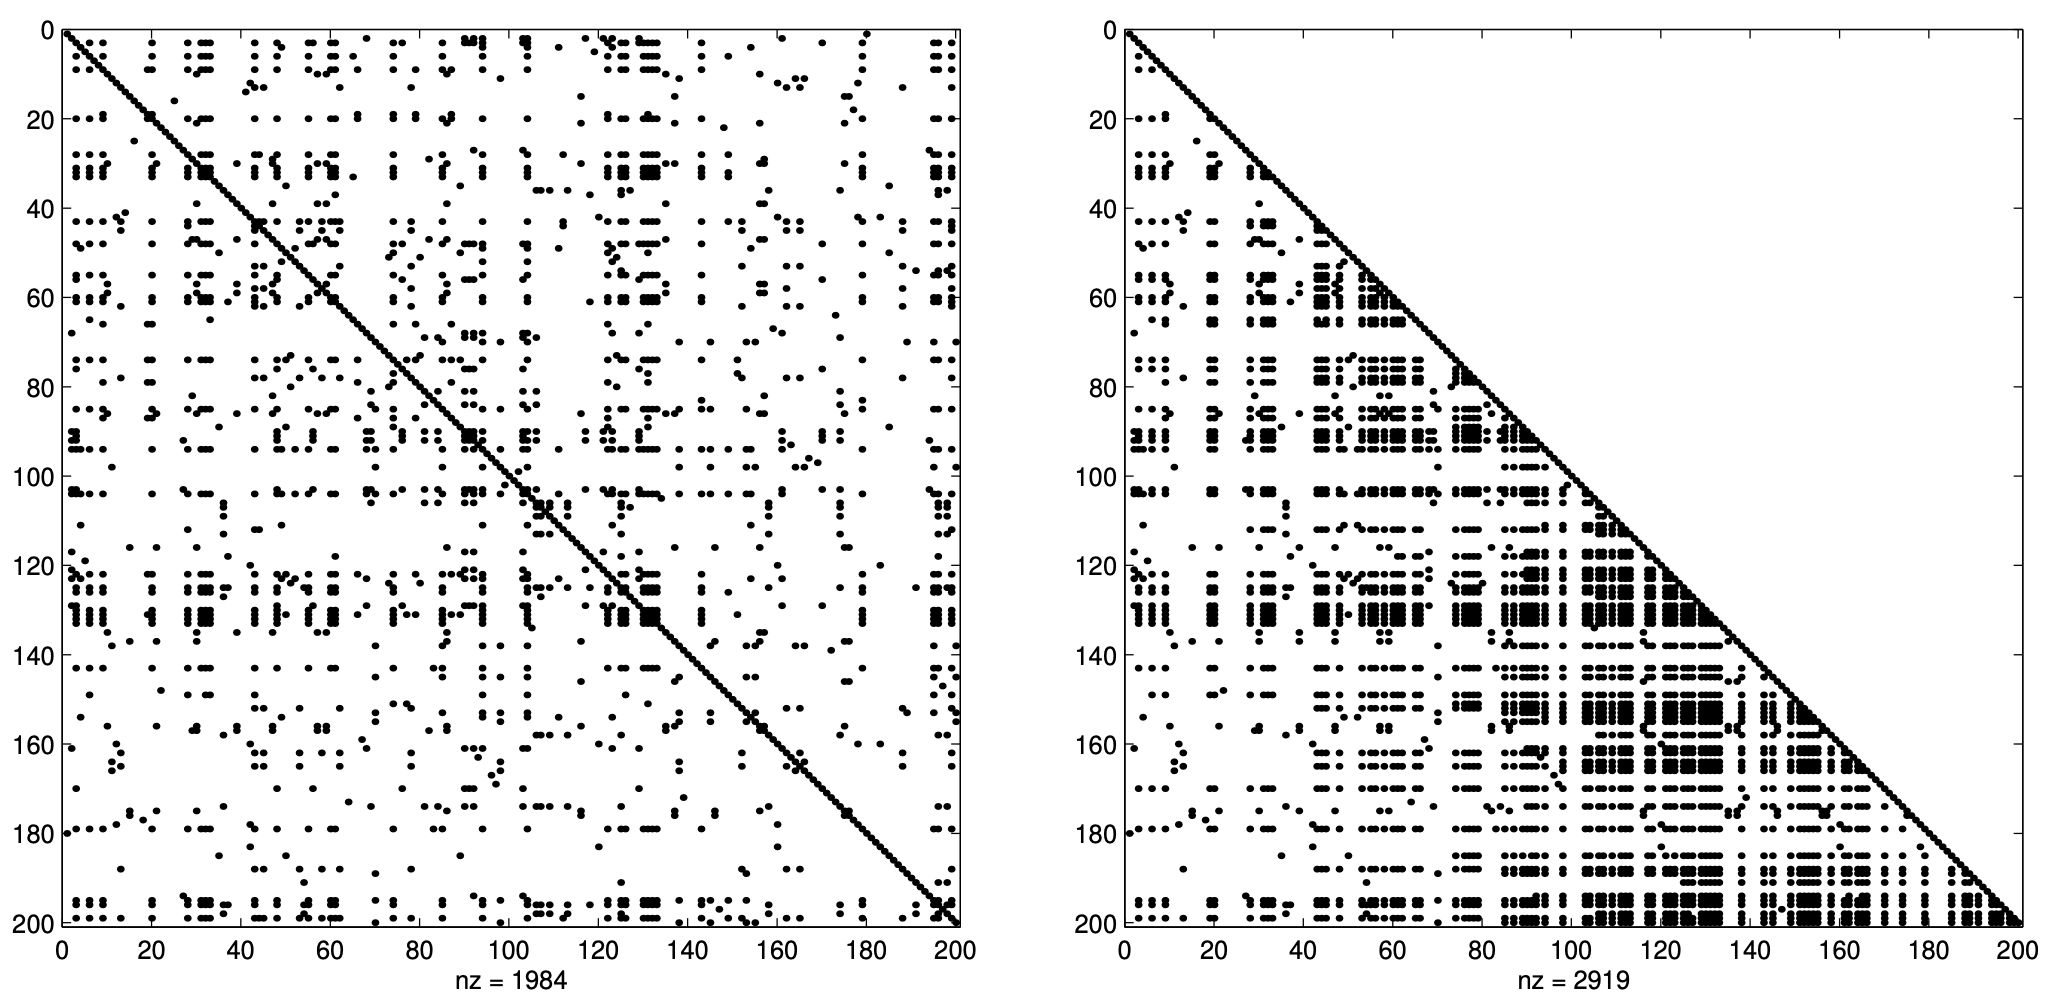
\includegraphics[width=0.6\textwidth]{Figures/matrix_storage.png}
    \caption{Sparsity pattern of $A$}
\end{figure}

Clearly $L$ is denser than $A$.

\begin{eg}
\[
A = 
\begin{pmatrix}
3 & 2 & 1 & 2 \\
2 & 4 & 0 & 0 \\
1 & 0 & 5 & 0 \\
2 & 0 & 0 & 6  
\end{pmatrix}
\]
\end{eg}

We will get a very dense $L$ if we do Cholesky factorization on $A$.
\[
    \text{chol}(A)
    =
    \begin{pmatrix}
        1.7321 &        0 &        0  &     0\\
        1.1547 &   1.6330 &        0  &     0\\
        0.5774 &  -0.4082 &   2.1213  &     0\\
        1.1547 &  -0.8165 &  -0.4714  &1.9437
    \end{pmatrix}
\]

If we do the reordering
\[
    P = \begin{pmatrix}
        0 & 0 & 0 & 1 \\
0 & 0 & 1 & 0 \\
0 & 1 & 0 & 0 \\
1 & 0 & 0 & 0  
    \end{pmatrix}, \quad AP^T = \begin{pmatrix}
        2 & 1 & 2 & 3 \\
  0 & 0 & 4 & 2 \\
  0 & 5 & 0 & 1 \\
  6 & 0 & 0 & 2
    \end{pmatrix}
\]

\[
PAP^T = 
\begin{pmatrix}
0 & 0 & 0 & 1 \\
0 & 0 & 1 & 0 \\
0 & 1 & 0 & 0 \\
1 & 0 & 0 & 0  
\end{pmatrix}
\begin{pmatrix}
  2 & 1 & 2 & 3 \\
  0 & 0 & 4 & 2 \\
  0 & 5 & 0 & 1 \\
  6 & 0 & 0 & 2
\end{pmatrix} =
\begin{pmatrix}
  6 & 0 & 0 & 2 \\
  0 & 5 & 0 & 1 \\
  0 & 0 & 4 & 2 \\
  2 & 1 & 2 & 3
\end{pmatrix}
\]

Then we get \[
\text{chol}(PAP^T) = \begin{pmatrix}
    2.4495 &        0&         0&         0\\
         0 &   2.2361&         0&         0\\
         0 &        0&    2.0000&         0\\
    0.8165 &   0.4472&    1.0000&    1.0646
\end{pmatrix}
\]

When we done the reordering, the $\text{chol}(PAP^T)$ is much sparser. Next we solve the original system $Ax = b$ by \[
    (PAP^T)Px = Pb
\]
Get $Px$ first, then get $x$.

The MATLAB provides method such as \begin{itemize}
    \item Column Count Reordering
    \item Reverse Cuthill-McKee Reordering
    \item Minimum Degree Reordering
    \item Nested Dissection Permutation
\end{itemize}

\begin{remark}
    In pratice, minimum fill-in problem is NP-hard, which is a combinatorial optimization problem, we can only get an approximation solution by some heuristics.
\end{remark}

However, minimum fill-in may not be the best: we need to consider the numerical stability, implementation efforts. Maybe finding a good reordering is more complicated than just doing the factorization and solve the system.
